\documentclass{biophys_letter}
\usepackage{dcolumn,color,helvet,times}
\usepackage{amsmath,lastpage,bm,textcomp}%mathtime
\usepackage{multicol}
\usepackage{cite} % my own added packages
\jno{kxl014} %journal number
\gridframe{N}%option for grid around the text "Y" or "N"
\cropmark{N}%option for cropmark around the text "Y" or "N"
        
\doi{doi: XX.XXXX/biophysj.XXX.XXXXXX}% DOI number in the copyright line
 
\begin{document}

\setcounter{page}{1} %first page number
\title{Statistical Inference for Nanopore Sequencing}

\author{Kevin Emmett,{\authdagger} Jacob Rosenstein, Jan-Willem van de Meent, Ken Shepard, and Chris Wiggins}

\address{{\addrdagger}Department of Physics and Department of Applied Physics and Applied Math, Columbia University, New York, New York; and Department of Mechanical Engineering, Brown University, Providence, Rhode Island}

\maketitle

\pagestyle{headings}

\markboth{Biophysical Journal: Biophysical Letters}{Biophysical Journal: Biophysical Letters} %for running head

%Abstract environment needs 3 arguments. They are
%1. The abstract
%2. Received date
%3. Address, email

\begin{abstract}
{DNA translocation through a nanopore is modeled as a one-dimensional biased random walk. A Hidden Markov Model is used to infer the input DNA sequence from a set of output read sequences. Bounds on inference accuracy are set based on model parameters.}
{Received for publication 1 April 2013 and in final form 1 April 2013.}
{*Correspondence: kje@phys.columbia.edu.}
\end{abstract}

\vspace*{2.7pt}

\begin{multicols}{2}
The pending transition of DNA sequencing platforms from today's ensemble measurements to upcoming single-molecule platforms has a variety of interesting bioinformatics consequences.
To date, all commercial sequencing platforms have relied on measurements of large sets of nominally identical molecules.
As a result, read lengths and nucleotide incorporation rates are commonly limited by the degree of synchronization that can be enforced among a population of nucleic acids.
At the single-molecule level such coordination is irrelevant, potentially allowing extremely fast reads of long contiguous sequences.
However, practical implementations of single-molecule sequencing introduce new sources of measurement error that should be considered carefully.

Nanopore sequencing is one platform which has emerged as a candidate for next-generation sequencing platforms \cite{Branton:2008}.
A number of strategies for sequencing DNA with nanopores have been proposed, with the common basis of detecting individual nucleotides as they pass through a nanometer-scale aperture in a thin membrane separating two electrolytes.
To date, a primary obstacle of this approach has been overcoming the fast stochastic motion of the individual molecules as they are driven through the pore \cite{Venkatesan:2011, Lu:2011}.
While recent methods have been proposed in order to controllably 'ratchet' DNA molecules through a nanopore one base at a time, experimental results show that motion of the molecule can still occur in both forward and backward directions within a single read \cite{Luan:2011, Olasagasti:2010, Cherf:2012}.
Therefore, unidirectional stepwise motion remains difficult to reliably achieve, leading to a novel source of error in the sequence read due to this diffusive motion.

In this letter, we demonstrate a statistical method of combining multiple reads from a given input DNA sequence passing through a nanopore that is able to yield highly accurate sequencing, even in the presence of highly diffusive molecular motion.
We consider a simple physical model of DNA translocation as a one-dimensional biased random walk, and demonstrate the use a Hidden Markov Model (HMM) to obtain a statistical estimate of the most likely input DNA sequence generating the observed series of reads.
We then use this model to set bounds on the achievable inference accuracy as a function of experimental parameters.
We conclude that multiple parallel reads are sufficient to compensate for both highly diffusive motion and high base-call error rates.

Translocation through the nanopore is modeled as a one-dimensional diffusion with driving force $F$ and unit base step size $a$, which we treat as a biased random walk with fixed forward bias $p$ \cite{Berg:1993}, where $p$ is given by
\begin{equation}
p = \frac{1}{2} + \frac{Fa}{4k_{B}T}.
\end{equation}
Given an input DNA sequence of length $L$, we generate a single output read of the sequence by stepping through the sequence with a bias $p$, at each step making a base call with error probability $e$.
Note that this error rate is strictly due to the base call and is independent of errors introduced due to backward motion. 
From this simple physical model, we generate a set of $N$ observed reads, each with length $T^{n} \ge L$ and denoted $X^n_{1:T_n}$.
A representation of the experimental configuration is shown in Figure \ref{fig:fig1}.

\end{multicols}

\twocolumn
\begin{figure}\vspace*{3pt}
  \centering{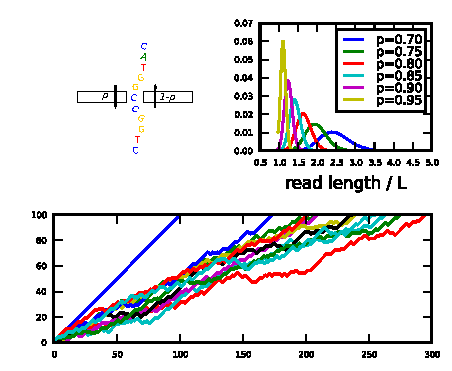
\includegraphics[width=3.25in]{fig/fig1.pdf}}
\caption{(A) Example of nanopore sequencing. (B) Example of random walks. (C) How data is generated}
\label{fig:fig1}
\end{figure}

Given this set of $N$ read sequences, the statistical task is to infer the true sequence most likely to have generated the observed data.
We model the data as a Hidden Markov Model (HMM) \cite{Rabiner:1989}, where each output read is modeled as a discrete set of observed states, $\mathbf{x}=\{x_{1}\dots x_{T}\}$, $x_i \in (A,G,C,T)$, a vector of observed bases, and a discrete set of hidden states, $\mathbf{z}=\{z_{1} \dots z_{T}\}$, $z_i \in (1 \dots L)$, the unknown position along the sequence.
For an HMM, we require three model parameters, the initial state distribution $\pi=p(\mathbf{z}_{1})$, the state transition matrix $A=p(\mathbf{z}_{t}|\mathbf{z}_{t-1})$, and an emission distribution $S=p(\mathbf{x}_{n}|\mathbf{z}_{n})$. 
$\pi$ and $A$ are taken as fixed given the experimental conditions, and our attention focuses on optimizing $p(\mathbf{x}_{n}|\mathbf{z}_{n})$, which directly represents our true sequence inference.
We maximize the complete data log likelihood, $p(X,Z|\theta)$, with respect to the model parameters using an implementation of expectation-maximization (EM).
Because the likelihood factorizes over the independent output reads, $p(X,Z|\theta)=\prod_{n}p(X^n,Z^n|\theta)$, we can perform expectation updates on each read individually before averaging results in the maximization step.
This key point provides us with a method of jointly using the all the information provided in the reads while still maintaing an efficient, parallel calculation.
After a convergence criteria on the complete data log likelihood is satisfied, we recover an estimated emission distribution $S$, which can be converted to an estimate for the DNA sequence by taking $\mathrm{\max_{d}} {S_{dl}}$.
The algorithm has complexity $O(L^{3})$.
An example of the output of this algorithm showing the relationship between the true sequence and the inferred sequence distribution is shown in Figure X.
Additionally, the column-wise entropy of the sequence inference is shown in Figure X(c). (to make)

We examined the performance of the algorithm over a range of parameter values in order to identify a minimal experimental configuration capable of sequence inference at a given accuracy.
First, we consider how to select realistic values for our parameters.
$p=0.5$ corresponds to completely symmetric diffusion and is unlikely to reach the end of the sequence.
$p=1.0$ corresponds to nondiffusive motion and is a trivial case in this model.
Real experiments will operate somewhere in between.
Lu et al. report an experimental bias term of $Fa/4k_{B}T=0.2$, for which they claim accurate sequence recovery is impossible \cite{Lu:2011}.
We take this as a starting point for investigation, exploring the range $p=0.7$ to $p=1.0$.
We are unsure of an appropriate base-call error rate, so we examine the full range $e=0.0$ to $e=0.5$.
The number of reads, $N$, is potentially unlimited.
A sweep across these parameters is shown in Figure X.
We observe that, as expected, the strongest determinant of achievable sequence accuracy is the number of reads, $N$.
This is expected because each read contributes an independent observation of the input DNA sequence.
We are most interested in the relationship between forward bias and the number of reads.
We observe an inference error rate that falls rapidly with increasing $N$, even at highly diffusive motion. 
If we set a threshold for performance at 99\% sequence accuracy, as measured in edit distance, we.
Figure \ref{fig:parameter_sweeps} shows the expected number of reads required to achieve a 98\% sequence accuracy, as measured by edit distance, as a function of the forward bias.
At current experimental limits, 98\% sequence accuracy is reliably achievable with $N=100$ at $p=0.7$ (figure doesn't really show this).
Finally, we observe that even high base-call error rates have minimal effect on inference accuracy, provided sufficient multiple reads are provided for averaging.

% figure 3: parameter sweeps
\begin{figure}%\vspace*{3pt}
  \centering{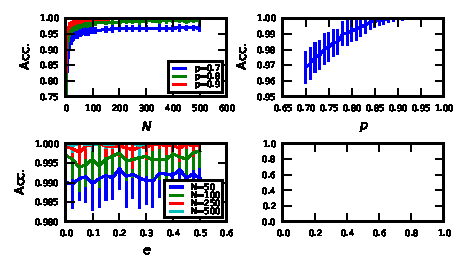
\includegraphics[width=3.25in]{fig/fig3.pdf}}
\caption{Parameter Sweeps. We plot inference accuracy (measured as 1 - edit distance/length) as a function of experimental parameters. (A) N vs P. (B) N vs P. (C) e vs N. (D) N vs e.}
\label{fig:parameter_sweeps}
\end{figure}

We next applied the method to fragments of $\lambda$-phage DNA.
We observe that, contrary to random DNA, the addition of more reads was often unable to bring the accuracy to 100\%.
We determined that this is due to specific sequence patterns that are more difficult for the algorithm to correctly parse, suggesting that a more specific method of identifying backwards motion may be required.

Next, we observe that errors in the sequence inference due to diffusive motion can take the form of extraneous insertions and deletion along the true sequence.
These errors are not random, but have a predictable pattern that makes it possible to identify and correct them during the inference algorithm.
This type of error occurs when there are multiple paths that may explain the observed data, and manifest themselves in the inference estimate as regions of higher entropy.
We used this observation to develop a heuristic that, acting after an initial maximum likelihood convergence, locates regions of high entropy, randomly introduces shifts in the sequence estimate, and restarts EM inference.
If the shifted inference yields a higher log likelihood, it is kept as explaining the data better than the previous estimate.
The procedure is repeated until no high entropy regions remain.
The procedure is detailed in Figure \ref{fig:entropy_restarts} on a segment of $\lambda$-phage DNA.

% figure 4: entropy heuristic
\begin{figure}
  \centering{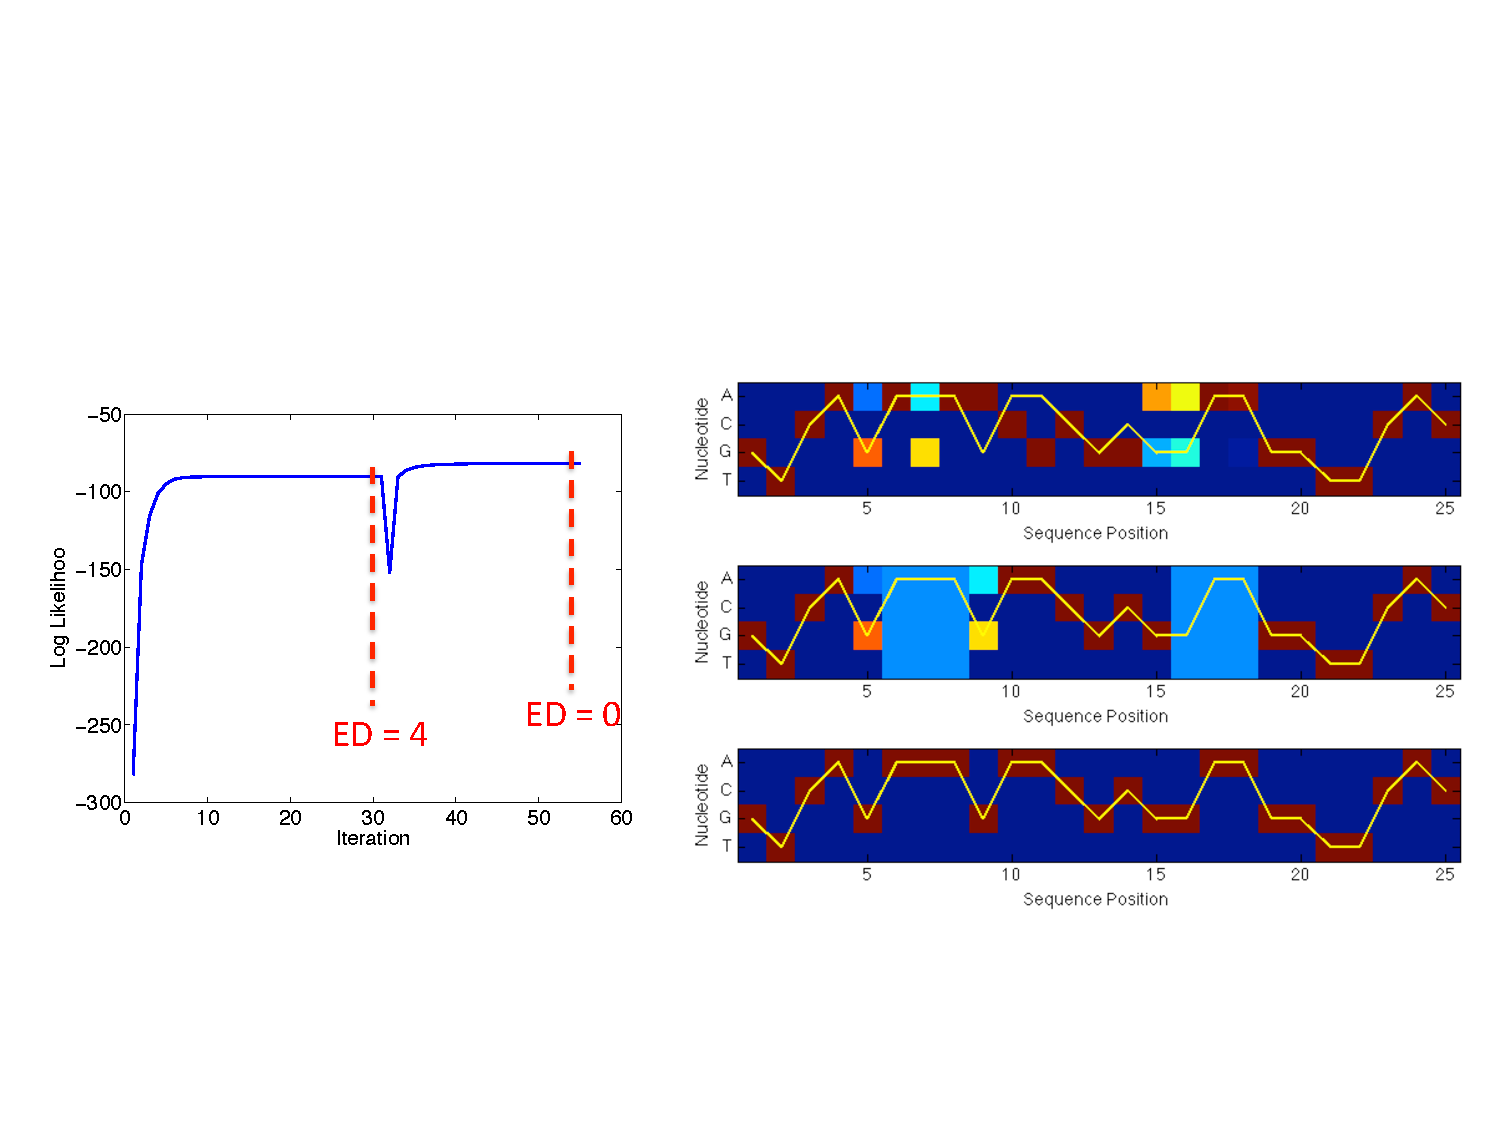
\includegraphics[width=3.25in]{fig/fig4.pdf}}
\caption{Restarts using entropy heuristic}
\label{fig:entropy_restarts}
\end{figure}

We have demonstrated a statistical method for inferring the DNA sequence passing through a nanopore sequencer under diffusive motion.
The strength of the method lies in the way in which multiple reads of the input sequence are independently modeled and then iteratively combined to yield a joint estimate of the true sequence.
Under this model, accurate sequence inference is achievable even within the experimental constraints of today's nanopore sequencers. ($p \approx 0.7$).
Designers of nanopore sequencers may find that there is a tradeoff between sequencing speed and maintaining unidirectional motion of the molecules.
In this scenario, techniques such as the random walk model may allow increased throughput without a loss of accuracy.

\section*{SUPPLEMENTARY MATERIAL}

A full derivation of the model and additional supplementary material can be found by visiting BPJ Online at http://www.biophysj.org.\vspace*{6pt}

\section*{ACKNOWLEDGEMENTS}

We acknowledge useful discussions with David Blei and David Pfau. Funding blurb.

\begin{thebibliography}{99}

\bibitem{Branton:2008}
  Branton, D., Deamer, D. W., Marziali, A., Bayley, H., Benner, S. A., Butler, T., et al.
  2008.
  The potential and challenges of nanopore sequencing.
  {\it Nat. Biotechnol.}
  26: 1146-–1153.
  doi:10.1038/nbt.1495

\bibitem{Venkatesan:2011}
  Venkatesan, B. M., and Bashir, R.
  2011.
  Nanopore sensors for nucleic acid analysis.
  {\it Nat. Nanotechnology.}
  6:615–-624.
  doi:10.1038/nnano.2011.129

\bibitem{Lu:2011}
  Lu, B., F. Albertorio, D.P. Hoogerheide, and J.A. Golovchenko.
  2011.
  Origins and consequences of velocity fluctuations during DNA passage through a nanopore.
  {\it Biophys J.}
  101:70–-79.
  doi:10.1016/j.bpj.2011.05.034

\bibitem{Luan:2011}
  Luan, B., H. Peng, S. Polonsky, S. Rossnagel, G. Stolovitzky, et al.
  2010.
  Base-by-base ratcheting of single stranded DNA through a solid-state nanopore.
  {\it Phys. Rev. Lett.}
  104:238103.
  doi:10.1103/PhysRevLett.104.238103

\bibitem{Olasagasti:2010}
  Olasagasti, F., K.R. Lieberman, S. Benner, G.M. Cherf, J.M. Dahl, et al.
  2010.
  Replication of individual DNA molecules under electronic control using a protein nanopore.
  {\it Nat. Nanotech.}
  5:798–806.
  doi:10.1038/nnano.2010.177

\bibitem{Cherf:2012}
  Cherf, G.M., K.R. Lieberman, H. Rashid, C.E. Lam, K. Karplus, et al.
  2012.
  Automated forward and reverse ratcheting of DNA in a nanopore at 5{\AA} precision.
  {\it Nat. Biotechnol.}
  30:344--348.
  doi:10.1038/nbt.2147

\bibitem{Berg:1993}
  Berg, H.C.
  1993.
  Random Walks in Biology.
  Princeton University Press.
  Princeton, New Jersey.

\bibitem{Rabiner:1989}
  Rabiner, L.R.
  1989.
  A tutorial on hidden Markov models and selected applications in speech recognition.
  {\it Proc. IEEE.}
  77:257-–286.
  doi:10.1109/5.18626

\bibitem{Dempster:1977}
  Dempster, A.P., N.M. Laird, and D.B. Rubin.
  1977.
  Maximum likelihood from incomplete data via the EM algorithm.
  {\it J. R. Statist. Soc. B.}
  39:1-–38.

\end{thebibliography}

%\end{multicols}
\end{document}
